\documentclass[12t,letterpaper]{article}

\newenvironment{proof}{\noindent{\bf Proof:}}{\qed\bigskip}

\newtheorem{theorem}{Theorem}
\newtheorem{corollary}{Corollary}
\newtheorem{lemma}{Lemma} 
\newtheorem{claim}{Claim}
\newtheorem{fact}{Fact}
\newtheorem{definition}{Definition}
\newtheorem{assumption}{Assumption}
\newtheorem{observation}{Observation}
\newtheorem{example}{Example}
\newcommand{\qed}{\rule{7pt}{7pt}}

\newcommand{\assignment}[4]{
\thispagestyle{plain} 
\newpage
\setcounter{page}{1}
\noindent
\begin{center}
\framebox{ \vbox{ \hbox to 6.28in
{\bf EE 126: Probability and Random Processes \hfill #1}
\vspace{4mm}
\hbox to 6.28in
{\hspace{2.5in}\large\mbox{#2}}
\vspace{4mm}
\hbox to 6.28in
{{\it Handed Out: #3 \hfill Due: #4}}
}}
\end{center}
}

\newcommand{\solution}[3]{
\thispagestyle{plain} 
\newpage
\setcounter{page}{1}
\noindent
\begin{center}
\framebox{ \vbox{ \hbox to 6.28in
{\bf EE 126 \hfill #3}
\vspace{4mm}
\hbox to 6.28in
{\hspace{2.5in}\large\mbox{#2}}
\vspace{4mm}
\hbox to 6.28in
{#1 \hfill}
}}
\end{center}
\markright{#1}
}

\newenvironment{algorithm}
{\begin{center}
\begin{tabular}{|l|}
\hline
\begin{minipage}{1in}
\begin{tabbing}
\quad\=\qquad\=\qquad\=\qquad\=\qquad\=\qquad\=\qquad\=\kill}
{\end{tabbing}
\end{minipage} \\
\hline
\end{tabular}
\end{center}}

\def\Comment#1{\textsf{\textsl{$\langle\!\langle$#1\/$\rangle\!\rangle$}}}


\usepackage{amsmath, dsfont, mathtools, verbatim, tikz, float}

\usetikzlibrary{arrows,automata}

\oddsidemargin 0in
\evensidemargin 0in
\textwidth 6.5in
\topmargin -0.5in
\textheight 9.0in

\newenvironment{amatrix}[1]{%
  \left(\begin{array}{@{}*{#1}{c}|c@{}}
}{%
  \end{array}\right)
}

\DeclarePairedDelimiter{\ceil}{\lceil}{\rceil}

\makeatletter
\renewcommand*\env@matrix[1][*\c@MaxMatrixCols c]{%
  \hskip -\arraycolsep
  \let\@ifnextchar\new@ifnextchar
  \array{#1}}
\makeatother

\newcommand{\norm}[1]{\left\lVert #1 \right\rVert}
\newcommand{\abs}[1]{\left\vert #1 \right\vert}
\newcommand{\?}{\stackrel{?}{=}}
\newcommand\given[1][]{\:#1\vert\:}
\renewcommand{\d}[1]{\ensuremath{\operatorname{d}\!{#1}}}

\begin{document}

\solution{Nikhil Unni}{HW6}{Spring 2016}
\pagestyle{myheadings}

\begin{enumerate}
  \item Consider the Markov chain with state $X_n, n \geq 0$, shown in Figure 1 (not pictured), where $\alpha, \beta \in (0,1)$.
    \begin{enumerate}
      \item Find the probability transition matrix $P$ and the invariant distribution $\pi$ of the Markov chain.\\\\

        We easily know what the transition matrix P is from the diagram:
        $$
        P = 
        \begin{pmatrix}[cc]
          1-\alpha & \alpha\\
          \beta    & 1-\beta\\
        \end{pmatrix}        
        $$

        Next, we can solve $\pi$ through the linear system of equations for the invariant property of $\pi P = \pi$:
        $$x(1-\alpha) + y \beta = x$$
        $$x + y = 1$$
        The original system of equations happens to be under constrained, so we can add on the fact that we know that the sum of the probabilities in the distribution is 1. Solving this system of equations we get:
        $$\pi = [\frac{-\beta}{\beta - \alpha}, \frac{2 \beta - \alpha}{\beta - \alpha}]$$

      \item Find two real numbers $\lambda_1$ and $\lambda_2$ such that there exists two non-zero vectors $u_1$ and $u_2$ s.t. $Pu_i = \lambda_iu_i$ for $i = 1,2$. Further, show that $P$ can be written as $P = UVU^{-1}$, where $U$ and $V$ are 2x2 matrices and $V$ is a diagonal matrix.\\\\

        We know eigenvectors/eigenvalues are the form $Pu = \lambda u$, which is equivalent to $(P - \lambda I)u = 0$. Since the $u$ we need are nonzero, we know that the determinant of $P - \lambda I$ must be 0. So we get:
        $$
        \det(
        \begin{pmatrix}[cc]
          1-\alpha-\lambda & \alpha\\
          \beta    & 1-\beta-\lambda\\
        \end{pmatrix}        
        )
        = \textbf{0}
        $$
        Expanding the determinant as a polynomial, and grouping like-terms together we get:
        $$\lambda^2 + \lambda(\beta + \alpha - 2) + (-\alpha - \beta + 1) = 0$$
        Solving with the quadratic formula, we get two values:
        $$\lambda_1 = 1, \lambda_2 = 1 - \alpha - \beta$$
        Plugging this back into our original two matrices we get:
        $$
        \begin{pmatrix}[cc]
          1-\alpha-1 & \alpha\\
          \beta    & 1-\beta-1\\
        \end{pmatrix}
        \textbf{x}
        =
        \textbf{0}
        $$
        Expanding this out, we get that $x=y$, so then we know $u_1 = [1/2, 1/2]^T$. For the other eigenvector we get:
        $$
        \begin{pmatrix}[cc]
          \beta & \alpha\\
          \beta & \alpha\\
        \end{pmatrix}
        \textbf{x}
        =
        \textbf{0}
        $$
        Solving this with the additional constraint that $x + y = 1$, we can get a solution:
        $$u_2 = [\frac{-\alpha}{\beta - \alpha}, \frac{\beta}{\beta - \alpha}]^T$$

        Let's let:
        $$U = [u_1,u_2]$$
        $$
        V 
        =
        \begin{pmatrix}[cc]
          \lambda_1 & 0\\
          0 & \lambda_2\\
        \end{pmatrix}
        $$

        Solving for $U^{-1}$ using the straightforward 2x2 inverse formula we get:
        $$
        U^{-1}
        =
        \frac{1}{\alpha + \beta}
        \begin{pmatrix}[cc]
          2 \beta & 2 \alpha\\
          \alpha - \beta & \beta - \alpha\\
        \end{pmatrix}        
        $$
        Manually multiplying out we get:
        $$
        UV
        =
        \begin{pmatrix}[cc]
          1/2 & -\frac{\alpha^2 + \alpha \beta - \alpha}{\alpha - \beta}\\
          1/2 & \frac{\beta^2 + \alpha \beta - \beta}{\alpha - \beta}\\
        \end{pmatrix}        
       $$
       And then multiplying with $U^{-1}$ we get:
       $$
       (UV)U^{-1}
       =
       \frac{1}{\alpha + \beta}
       \begin{pmatrix}[cc]
         1/2 & -\frac{\alpha^2 + \alpha \beta - \alpha}{\alpha - \beta}\\
         1/2 & \frac{\beta^2 + \alpha \beta - \beta}{\alpha - \beta}\\
       \end{pmatrix}        
        \begin{pmatrix}[cc]
          2 \beta & 2 \alpha\\
          \alpha - \beta & \beta - \alpha\\
        \end{pmatrix}               
       $$
       $$
       =
       \begin{pmatrix}[cc]
         1 - \alpha & \alpha\\
         \beta & 1 - \beta\\
       \end{pmatrix}
       =
       P
       $$

     \item Find $P^n$ in terms of $U$ and $V$.\\\\

       Notice that $P^2 = (UVU^{-1})(UVU^{-1}) = UVVU^{-1} = UV^2U^{-1}$. Continuing in this pattern, notice that:
       $$P^n = UV^nU^{-1}$$

     \item Assume that $X_0 = 0$. Use the result in part (c) to compute the PMF of $X_n$ for all $n \geq 0$. Verify that it converges to the invariant distribution.\\\\

       Since diagonal matrices are merely ``scaling'' for each of the dimensions, $V^n$ should just be all of the individual eigenvalues raised to the n. This gives us:
       $$
       V^n
       =
       \begin{pmatrix}[cc]
         1 & 0\\
         0 & (1-\alpha-\beta)^n\\
       \end{pmatrix}
       $$

       Then:
       $$
       UV^n
       =
       \begin{pmatrix}[cc]
         1/2 & \frac{-\alpha}{\beta - \alpha}\\
         1/2 & \frac{\beta}{\beta - \alpha}\\
       \end{pmatrix}       
       \begin{pmatrix}[cc]
         1 & 0\\
         0 & (1-\alpha-\beta)^n\\
       \end{pmatrix}
       =
       \begin{pmatrix}[cc]
         1/2 & \frac{-\alpha(-\alpha - \beta + 1)^n}{\beta - \alpha}\\
         1/2 & \frac{\beta(-\alpha - \beta + 1)^n}{\beta - \alpha}\\
       \end{pmatrix}      
       $$
       And:
       $$
       (UV^n)U^{-1}
       =
       \frac{1}{\alpha + \beta}
       \begin{pmatrix}[cc]
         1/2 & \frac{-\alpha(-\alpha - \beta + 1)^n}{\beta - \alpha}\\
         1/2 & \frac{\beta(-\alpha - \beta + 1)^n}{\beta - \alpha}\\
       \end{pmatrix}
       \begin{pmatrix}[cc]
         2 \beta & 2 \alpha\\
         \alpha - \beta & \beta - \alpha\\
       \end{pmatrix}        
       =
       \begin{pmatrix}[cc]
         \beta + \alpha(-\alpha-\beta+1)^n & \alpha - \alpha(-\alpha - \beta + 1)^n\\
         -\beta(-\alpha-\beta+1)^n & \alpha + \beta (-\alpha - \beta + 1)^n\\
       \end{pmatrix}       
       $$
       
       Finally:
       $$[1,0] * UV^nU^{-1} = \frac{1}{\alpha + \beta} [\beta + \alpha(-\alpha-\beta+1)^n, \alpha - \alpha(-\alpha - \beta + 1)^n]$$
       
    \end{enumerate}

  \item A discrete-time Markov chain with seven states has the following transition probabilities (not shown)\\

    In the questions below, the $X_k$ be the state of the Markov chain at time k.
    \begin{enumerate}
      \item Give a pictorial representation of the dicsrete-time Markov chain.\\\\
        \begin{figure}[H]
        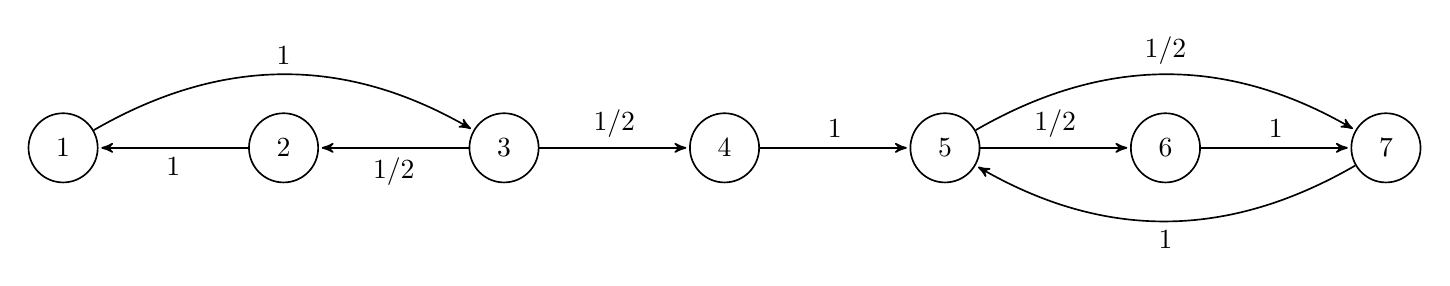
\begin{tikzpicture}[->,>=stealth',shorten >=1pt,auto,node distance=2.8cm, semithick]
          \tikzstyle{every state}=[fill=none,draw=black,text=black]
          \node[state]         (1)              {1};
          \node[state]         (2) [right of=1] {2};
          \node[state]         (3) [right of=2] {3};
          \node[state]         (4) [right of=3] {4};
          \node[state]         (5) [right of=4] {5};
          \node[state]         (6) [right of=5] {6};
          \node[state]         (7) [right of=6] {7};

          \path (1) edge [bend left]  node {1}   (3)
                (2) edge              node {1}   (1)
                (3) edge              node {1/2} (2)
                    edge              node {1/2} (4)
                (4) edge              node {1}   (5)
                (5) edge [bend left]  node {1/2} (7)
                    edge              node {1/2} (6)
                (6) edge              node {1}   (7)
                (7) edge [bend left]  node {1}   (5);

        \end{tikzpicture}
        \end{figure}

      \item For what values of $n$ is $P(X_n = 5 | X_0 = 1) > 0$?\\\\

        Starting from 1, notice that we can loop through 1,2,3 $3i, i \in \mathds{N}$ times before moving on. Then 1 hop to 3, 1 hop to 4, 1 hop to 5. From 5 we can repeat loops of 2 or 3. So the set of valid $n$ values are:
        $$n \in \{3i + 3 + 2j + 3k: i,j,k \in \mathds{N}\}$$

      \item What is the set of states $A(i)$ that are accessible from state $i$, for each $i = 1, \cdots, 7$? Is the Markov chain irreducible?\\\\

        $A(1) = \{1, \cdots, 7\}, A(2) = \{1, \cdots, 7\}, A(3) = \{1, \cdots, 7\}, A(4) = \{4, \cdots, 7\}, A(5) = \{5, \cdots, 7\}, A(6) = \{5, \cdots, 7\}, A(7) = \{5, \cdots, 7\}$.\\

        Because the sets are not all $\{1, \cdots, 7\}$, the chain is not irreducible.


      \item Identify which states are transient and which states are recurrent. For each recurrent state, state whether it is periodic (and give the period) or aperiodic.\\\\

        $4$ is transient, and the rest are recurrent. $1,2,3$ are periodic, and $5,6,7$ are aperiodic because $\gcd(2,3) = 1$.\\

      \item If $X_0 = 1$, what is the expected time for the Markov chain to reach state $7$ for the first time?\\\\

        Call the expected time to get to j from i $e_i(j)$. We know that $e_1(3)$ is just 1. From 3, there's a possibility of going around the 1-2-3 loop w.p. $\frac{1}{2}$ and w.p. $\frac{1}{2}$ we'll move on to 4. So we can say:
        $$e_1(4) = 1 + 3 \mathds{E}[\text{\# of loops}] + 1$$
        And notice that \# of loops ~ Geom($\frac{1}{2}$). So we know E[\# of loops] = 2. Then, $e_1(4) = 8$. Getting to 5 is obviously $e_1(5) = 9$. From 5, w.p. $\frac{1}{2}$ we have 2 time steps to $7$, and w.p. $\frac{1}{2}$ we have 1 time step to $7$. So $e_5(7) = \frac{1}{2}(2) + \frac{1}{2}(1) = 1.5$. Putting it all together we get:
        $$e_1(7) = 9 + 1.5 = 10.5$$
    \end{enumerate}

  \item You are playing a card game with your friend. You each have $m$ cards in your hand. Out of the $2m$ total cards, $m$ are green, and $m$ are blue. At each round, you and your friend each randomly select a card from your respective hands and switch cards.
    \begin{enumerate}
      \item Let $X_n$ be the number of blue cards you have in your hand after you and your friend have exchanged cards $n$ times. Find the transition probabilities for the Markov Chain $X_n$.\\\\

        At some time, say that I have $i$ blue cards. That means I have $m-i$ green, and my friend has $m-i$ blue and $i$ green. Let $P_{i \to\ j}$ be the probability of going from $i$ blue cards to $j$ blue cards. Then:
        $$P_{i \to\ i+1} = \text{P(I don't select blue)P(he selects blue)} = \frac{m-i}{m} \frac{m-i}{m} = \frac{(m-i)^2}{m^2}$$
        $$P_{i \to\ i-1} = \text{P(I select blue)P(he selects green)} = \frac{i}{m} \frac{i}{m} = \frac{i^2}{m^2}$$
        $$P_{i \to\ i} = \text{P(I select blue)P(he selects blue) + P(I select green)P(he selects green)}$$
        $$=\frac{m-i}{m} \frac{i}{m} + \frac{i}{m} \frac{m-i}{m} = \frac{2i(m-i)}{m^2}$$\\

      \item A reversible Markov Chain has the transition probabilities $Q_{ij} = \pi_j \frac{P_{ji}}{\pi_i}$ and a time reversible Markov Chain is such that $Q_{ij} = P_{ij}$. Show that the Markov Chain $X_n$ is time reversible.\\\\

        For the invariant distribution, or in the limit of the sequence, the ``flow'' into a node is equal to the ``flow'' out of the node. It's analogous to fluid flow wherein there's a constant amount of fluid in the system (in this case the total probability = 1), and so at each time step, the flow into a node has to be equal to the flow out of a node. This is true for irreducible and aperiodic Markov chains.\\

        But this concept can be extended to sets of nodes. If you group together sets of nodes, and only think about probabilities entering the set or exiting the set, this has to be conserved as well. You can think of it with the fluid analogy, or just modify the Markov chain by grouping together the set as one node, and adjust the probabilities in and out of the set accordingly.\\

        So for some node $i$, create a cluster of nodes $\{0, \cdots, i\}$. So the only flow coming in has to be from node $i+1$, and the flow out has to be the flow from $i$ to $i+1$. So we have:
        $$\text{Flow into set = Flow out of set}$$
        $$P_{i+1 \to\ i} (\pi_{i+1}) = P_{i \to\ i+1} (\pi_{i})$$
        But just label $i+1$ as $j$, and we have:
        $$P_{ji} (\pi_{j}) = P_{ij} (\pi_{i})$$
        Or:
        $$\pi_j \frac{P_{ji}}{\pi_{i}} = P_{ij}$$
        
        This works backwards as well -- if for each node $i$, you create a cluster of nodes $\{i, \cdots, m\}$, you get:
        $$\text{Flow into set = Flow out of set}$$
        $$P_{i-1 \to\ i} (\pi_{i-1}) = P_{i \to\ i-1} (\pi_{i})$$
        And label $i-1$ as $j$:
        $$P_{ji} (\pi_{j}) = P_{ij} (\pi_{i})$$
        $$\pi_j \frac{P_{ji}}{\pi_{i}} = P_{ij}$$
        Since the equality holds in both directions, and there's no way to get to another node that isn't $i-1$ or $i+1$, and the equality obviously holds for transitions from $i \to\ i$, the Markov chain is time reversible.
        
    \end{enumerate}

  \item An ant is walking on the nonnegative integers. At each step, the ant moves forward one step with probability $p$, or slides back down to $0$ with probability $1-p$. What is the average time it takes for the ant to get to $n$?\\\\

    Call $e(k)$ the average time it takes to reach $n$ from state $k$. Notice that $e(0) = 1 + pe(1) + (1-p)e(0)$, or:
    $$e(0) = \frac{1}{p} + e(1)$$
    Also:
    $$e(1) = 1 + pe(2) + (1-p)e(0)$$
    Plugging in those values for our original we get:
    $$e(0) = \frac{1}{p} + 1 + pe(2) + (1-p)e(0)$$
    $$e(0) = \frac{1}{p^2} + \frac{1}{p} + e(2)$$

    Continuing on in this pattern, we see:
    $$e(0) = \Sigma_{i=1}^n \frac{1}{p^i} + e(n)$$
    And we know that $e(n) = 0$, since we've already reached the state. So we have:
    $$e(0) = \Sigma_{i=1}^n \frac{1}{p^i} = \frac{1-p^{-n}}{p-1}$$

  \item 
    \begin{enumerate}
      \item Find the steady-state probabilities $\pi_0, \cdots, \pi_{k-1}$ for the Markov chain in Figure 2 (not pictured). Express your answer in terms of the ratio $\rho = p/q$, where $q = 1-p$. Pay particular attention to the special case $\rho = 1$.\\\\

        Following the same flow idea from \#3, we can cluster sets of nodes together and look at the flow in and out of the set to get probabilities. Specifically, for each node $i$, we group $\{0, \cdots, i\}$, we get:
        $$\text{Flow out = Flow in}$$
        $$\pi_i (p) = \pi_{i+1} (1-p)$$
        $$\pi_{i+1} = \rho \pi_i$$
        Inducuctively, we see that for any node $i$, $\pi_i = \rho^i \pi_0$. We also know that the sum of the invariant probabilities is 1. So we get:
        $$\Sigma_{i=0}^{k-1} \rho^i \pi_0  = 1$$
        $$\pi_0 (\Sigma_{i=0}^{k-1} \rho^i) = 1$$
        $$\pi_0 (\frac{\rho^k-1}{\rho-1}) = 1$$
        Finally:
        $$\pi_0 = \frac{\rho-1}{\rho^k - 1}$$
        $$\pi_i = \frac{\rho-1}{\rho^k - 1} \rho^i$$

        In the special case of $\rho = 1$:
        $$\pi_0 (\Sigma_{i=0}^{k-1} \rho^i) = 1$$
        $$\pi_0 (k) = 1$$
        Then:
        $$\pi_0 = \frac{1}{k}$$
        $$\pi_i = \frac{1}{k}$$
      \item Find the limit of $\pi_0$ as $k$ approaches infinity; give separate answers for $\rho < 1$, $\rho = 1$, and $\rho > 1$. Find limiting values for $\pi_{k-1}$ for the same cases.\\\\\
        
        \begin{itemize}
          \item [$\rho > 1:$]
            $$\lim_{k \to\ \infty} \pi_0 = \frac{\rho - 1}{\infty - 1} = 0$$
            $$\lim_{k \to\ \infty} \pi_{k-1} = \lim_{k \to\ \infty} \frac{1 - \frac{1}{\rho}}{1 - \frac{1}{\rho^k}} = 1 - \frac{1}{\rho}$$
          \item [$\rho = 1$:]
            $$\lim_{k \to\ \infty} \pi_0 = \frac{1}{k}$$
            $$\lim_{k \to\ \infty} \pi_{k-1} = \frac{1}{k}$$
          \item [$\rho < 1$:]
            $$\lim_{k \to\ \infty} \pi_0 = \frac{\rho-1}{0-1} = 1-\rho$$
            $$\lim_{k \to\ \infty} \pi_{k-1} = \frac{0 - 0}{0 - 1} = 0$$
        \end{itemize}
    \end{enumerate}
      
\end{enumerate}

\end{document}
